\section{Task Definition} \label{modeling.task.def}
\begin{figure*}[!htb]
\begin{subfigure}{0.5\textwidth}
    \centering
    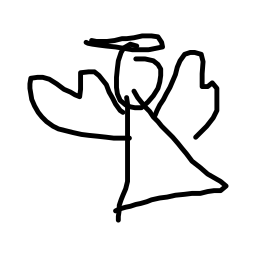
\includegraphics[width=0.5\linewidth]{modeling/angel340.png}
    \caption{$t_1$: \textit{wide triangular body}}
    \label{modeling.task.sketches.1}  
\end{subfigure}
\begin{subfigure}{0.5\textwidth}
    \centering
    
\includegraphics[width=0.5\linewidth]{modeling/angel389.png}   
    \caption{$t_2$: \textit{small rectangular body}}
    \label{modeling.task.sketches.2}  
\end{subfigure}
\caption{Two angel sketches, $s_1$ on the left and $s_2$ on the right, and their part annotations, $t_1$ and $t_2$. The task is for CLIP to determine which sketch matches a given $t_j$.}
\label{modeling.task.sketches}
\end{figure*}

% Since task should be method-independent, maybe mention that in this case we choose CLIP to do this task. This task can be done wtih any multimodal embeddings. 
Given two sketches $(s_1,s_2)$ and their part annotations $(t_1,t_2)$, such as the pair shown in Figure \ref{modeling.task.sketches}, the task is to determine which sketch $t_j$ should be paired with.
We use this task to evaluate the joint vision-language embedding space of CLIP, which is often used as part of the objective function for models that generate image from text; the objective function often involves maximizing the cosine similarity between the generated image and the provided text (or some variants engineered to work for the particular latent space of the generator used) \citep{clipDrawPaper,styleCLIPPaper,styleganNadaPaper,dalle2Paper}. 
Through this task, we can study how well CLIP can recognize different visual concepts in sketches, and the experiments can help us determine if CLIP can be used in similar ways to guide part-based sketch generation from language. Moreover, since we give CLIP the same pairs that were given to the annotators, we can learn if CLIP can understand how people are using language to describe the visual features of the sketches. 